\documentclass[11pt,letterpaper]{article}
\usepackage{array}
\usepackage[in]{fullpage}
\usepackage{verbatim}
\usepackage{parskip}
\usepackage{graphicx}

\usepackage{titlesec}
\titlespacing{\section}{0pt}{\baselineskip}{0pt}
\titleformat*{\section}{\normalsize\bfseries\MakeUppercase}

\titlespacing{\subsection}{0pt}{0.5\baselineskip}{0pt}
\titleformat*{\subsection}{\normalsize\bfseries}

%\setlength{\parindent}{0in}

% precede modeling with a short discussion of motivation behind modeling
% 1. understanding vs. prediction
% 2. complex is not necessarily better. elegant is best!

\begin{document}
\textbf{ENVS S422: Earth's Climate System\\
Modeling Exercise 2: Daisyworld}\\%\footnote{Based on exercises developed by Dave Bice at Penn State University.}}\\

Daisyworld is a simple toy model that was developed to show that feedbacks within the Earth system can have a stabilizing effect on Earth's climate. The planet consists of uncovered land, white daisies, and black daisies. The area covered by daisies can grow or shrink as Earth's temperature fluctuates. The temperature depends on the solar radiation and the albedo of the uncovered land and daisies. That's basically it. Daisyworld doesn't contain an atmosphere, oceans, ice sheets, or mountains.

For each model experiment, you should submit a brief 1-paragraph response to the questions that are being explored in the exercise and \textit{at least} one graph to help justify your response.

Due date: 11 February 2019

\section{Background to Daisyworld}
\subsection{Planetary temperature}
We will model Daisyworld by assuming that changes in the planet's energy budget are slow. Thus we can assume that the rate at which energy is emitted by the planet equals the rate at which it is absorbed. (Recall from the IPCC report that at present the Earth is currently gaining energy, and so there is an energy imbalance. However, the current energy imbalance is just a small percentage of the total energy being received by the Earth.) The rate at which energy is emitted is given by the Stefan-Boltzmann Law:
\begin{equation}
\left(\frac{dE}{dt}\right)_{\rm outgoing}=\sigma\epsilon AT^4,
\label{eq:stefan-boltzmann}
\end{equation}
where $\sigma=5.6704\times{10}^{-8}\mbox{ W/(m}^2\cdot\mbox{K}^4\mbox{)}$ is the Stefan-Boltzmann constant, $\epsilon$ is the emissivity, $A$ is the planet's surface area, and $T$ is temperature in kelvins. The emissivity is a dimensionless number between 0 and 1 that indicates how easily an object can emit energy. For simplicity, we will assume that $\epsilon=1$, so that Equation (\ref{eq:stefan-boltzmann}) becomes
\begin{equation}
\left(\frac{dE}{dt}\right)_{\rm outgoing}=\sigma AT^4,
\label{eq:stefan-boltzmann2}
\end{equation}
The rate at which energy is absorbed by the planet equals the rate at which energy is received from the sun minus the rate at which energy is reflected back into space
\begin{equation}
\left(\frac{dE}{dt}\right)_{\rm incoming}=IA-\left(\frac{dE}{dt}\right)_{\rm reflected},
\label{eq:absorbed1}
\end{equation}
\noindent where $I$ is the irradiance, or rate (i.e., flux) at which energy is received from the sun per unit area. The rate at which energy is reflected is determined by the planetary albedo, $\alpha$, so that
\begin{equation}
\left(\frac{dE}{dt}\right)_{\rm reflected}=\alpha{IA}.
\label{eq:reflected}
\end{equation} 
\noindent Albedo is a reflection coefficient between 0 and 1; when $\alpha=0$, none of the incoming radiation is reflected, and when $\alpha=1$, all of the incoming radiation is reflected. Combining Equations (\ref{eq:absorbed1}) and (\ref{eq:reflected}), we find that
\begin{equation}
\left(\frac{dE}{dt}\right)_{\rm incoming}=IA(1-\alpha).
\label{eq:absorbed2}
\end{equation}
Now, because we have assumed that the rates at which energy enters and leaves the planet are the same, we can equate Equations (\ref{eq:stefan-boltzmann2}) and (\ref{eq:absorbed2}) and divide by the surface area to find that
\begin{equation}
\sigma{T^4}=I(1-\alpha).
\end{equation}
Finally, rearranging gives
\begin{equation}
T=\left(\frac{I(1-\alpha)}{\sigma}\right)^{1/4}.
\end{equation}
Ultimately, this is the equation that we want to solve: How does Daisyworld's temperature vary with time? It depends on the irradiance, or incoming radiation from the sun, and the planetary albedo. The irradiance will be prescribed, while the albedo will depend on the growth of daisies, which depends on temperature. 


\subsection{Solar irradiance}
Daisyworld's sun begins with a diminished brightness (like all stars) and grows brighter with time. At the beginning of Daisyworld, it provides an irradiance of 550 $\mbox{W/m}^2$ to Daisyworld; two billion years later it provides 1650 $\mbox{W/m}^2$. (The Earth currently receives 1366 $\mbox{W/m}^2$.) We will prescribe this change in irradiance with a simple linear equation:
\begin{equation}
I=550+\frac{1100t}{200},
\end{equation}
\noindent where $t$ is time in 10 million years (i.e., each time step equals 10 million years).

\subsection{Planetary albedo}
The albedo of Daisyworld is a function of how much area is covered by white daisies and black daisies. Uncovered land has an albedo of 0.5, while white daisies and black daisies have albedos of 0.75 and 0.25, respectively. The net planetary albedo, $A$, is
\begin{equation}
\alpha=A_{u}\alpha_{u}+A_w\alpha_w+A_b\alpha_b,
\end{equation}
\noindent where $a_{u}$, $A_w$, and $A_b$ are the fraction of the total area that is uncovered, covered with white daisies, and covered with black daisies (so that $A_{u}+A_w+A_b=1$), and $\alpha_{u}$, $\alpha_w$, and $\alpha_b$ are the albedos of the uncovered land, white daisies, and black daisies.

The tricky part of this exercise is that the fractional areas will change with time, and the rate at which they change will depend on temperature. In particular, we will assume that the rate of fractional area change (for white daisies) is given by
\begin{equation}
\frac{d}{dt}A_w=A_w(g_w-d_w),
\end{equation} 
where $g_w$ and $d_w$ are the growth rate and death rate. This equation tells us that (1) if the growth rate exceeds the death rate, then the fractional area will increase, and (2) the rate of change depends on the area already covered by daisies. In other words, large amounts of daisies can die or be produced when the population is large. We will use an identical equation for black daisies.

For the death rate, we will simply use a constant value of 0.3. This is equivalent to saying that, given a growth rate of 0, the fractional area of each type of daisy will decrease by 30\% during each interval of time (10 million years).

The growth rate will depend on the local temperature near the daisies and the area of uncovered land, such that
\begin{equation}
g_w=A_u(1-0.003265(273+22.5-T_w)^2),
\label{eq:growthrate}
\end{equation}
\noindent where $T_w$ is the local temperature in the vicinity of the white daisies. This equation looks complicated, but in reality it is just a parabola. The growth rate equals 0 when the temperature is 5$^\circ$C (278 K) and 40$^\circ$C (313 K), and reaches a maximum when the temperature is 22.5$^\circ$C (295.5 K). Furthermore, the growth rate depends on the area of uncovered land. If there is a lot of bare land, the daisies can spread more rapidly. One problem with Equation (\ref{eq:growthrate}) is that it gives negative growth rates for temperatures less than 5$^\circ$C or greater than 40$^\circ$C. We will need to account for this by using a ``conditional'' statement in our model that will force the growth rate to equal 0 if the temperature isn't between 5$^\circ$C and 40$^\circ$C.

Finally, we want to account for the fact that the temperature near the white daisies will differ from the average global temperature. This will be calculated by
\begin{equation}
T_w=H_a(\alpha-\alpha_w)+T,
\end{equation}
\noindent where $H_a$ is a heat absorption factor. We will set $H_a=20$, which means that the temperature near the daisies will be 5$^\circ$C cooler than the average temperature on the planet (if $\alpha=0.5$ and $\alpha_w=0.75$).

These equations describing daisy growth and death are a bit arbitrary and only loosely based on studies of population biology. In other words, don't take them too seriously. However, we can easily play with the equations to see how changing the conditions under which daisies thrive affects the stability of Daisyworld. The point here isn't to get an accurate portrayal of reality --- and in fact, we've already neglected the atmosphere, the oceans, and nutrient cycling --- instead, we're just trying to get an idea of how systems work and how non-intuitive they can be.

\section{Numerical experiments}
For these experiments I am providing you with a pre-built STELLA model of Daisyworld (Fig. \ref{fig:daisyworld}). It is available on the course website. After each of the following experiments, you should return to the original model.

\begin{figure}[t]
\centering{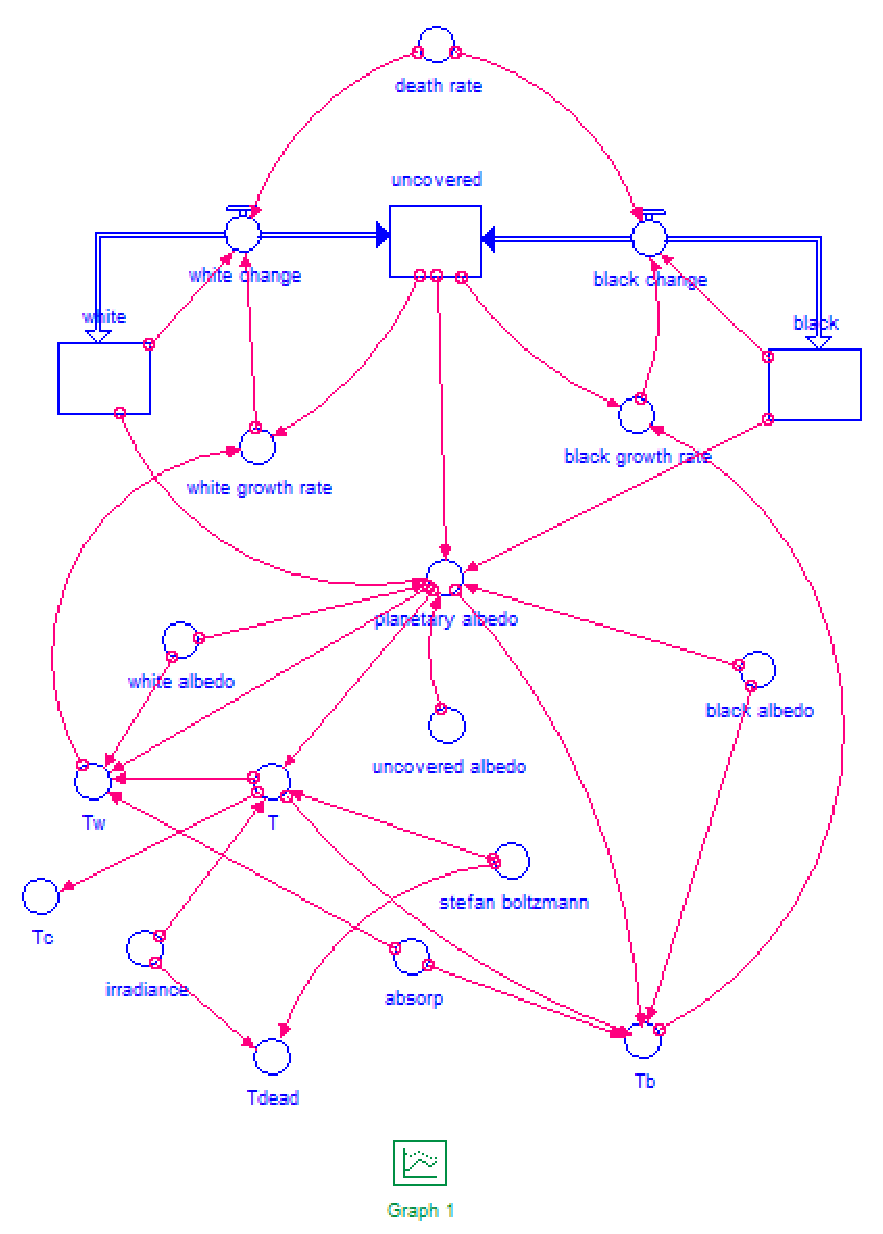
\includegraphics[width=3in]{./daisyworld}}
\caption{Screenshot of the Daisyworld model that you will explore.}
\label{fig:daisyworld}
\end{figure}

\subsection{Initial simulations}
You will begin with the model set-up as described above. Run the model for 200 time units, using a time step of 0.25 time units. It will be instructive to plot the three reservoirs on one graph, and the average planetary temperature and the temperature of a ``dead'' planet on another graph. Other graphs may be necessary to fully understand what is driving the observed behavior.

Describe how the daisies affect the planetary temperature? When do the daisies start to grow? Do both start growing at the same time? What type of daisies live the longest, and why? What happens if you set the black daisy growth rate to 0? What if you set the white daisy growth rate to 0?

\subsection{Varying the albedos}
Initially, the black albedo is set at 0.25, while the white albedo is 0.75. In this experiment, modify these albedos, first to more
extreme values (0.05 and 0.95) and then to more moderate values (0.4 and 0.6). Generate some comparative plots to show how these different scenarios influence the planetary temperature.

\subsection{Varying the growth factor curves}

One of the critical parts of this model is the growth factor for daisy growth. In this experiment, you will alter the growth factor and
see how the model responds.

(a) First, alter the optimum temperature for the daisies' growth, which is initially set at 22.5$^\circ$C, to 15$^\circ$C. To do this, alter the equations for the growth factors by replacing 22.5 with 15 and adjust the conditional statement so that the growth rate doesn't become negative (subtract 7.5 from both the minimum and maximum bounds). 

(b) Next, restore the optimum temperature to 22.5$^\circ$C and then reduce the range of temperatures that the daisies can tolerate. Initially,
the daisies can grow in temperatures ranging from 5 to 40. Now restrict the range so that the daisies grow only between 18 and 27;
this can be done by replacing the 0.003265 with 0.05 in the equations for the growth factors. As in the part (a), you will also need to adjust the conditional statement to ensure that the growth rate isn't negative outside of this temperature range. 

How do the optimum temperature for growth and the tolerable temperature range affect the planetary temperature?

\subsection{Plagues}
This experiment explores the resilience of Daisyworld by programming a set of plagues into the model. These plagues decimate the
populations periodically for brief periods. An interesting question here is whether or not the daisies will be able to recover fast
enough to return the planetary temperature to the ``comfort zone''. To implement this change, double-click on the death rate
converter and replace 0.3 with ``TIME'' (without the quotation marks), then click on the Graph button in the lower left of the
window, and check the ``graphical'' radio button. Next set the number of data points to 101; this should give you one input value every 2 time units, thus allowing us to make fairly brief plagues (still, these are 20 million years long!). Then, set the scale on the graph to 0.3, and click and drag the graph until all of the time steps have a death rate of 0.3. Next, click on the points tab, and manually change the death rate to a value of 1.0 at time units 50, 100, and 150 (and others, if you'd like); click on the OK button and the plagues should be inserted into the model. Run the model as before, after making a prediction about what will happen. 

Are all of the plagues equal in magnitude (in terms of area lost as a result of the deaths)? Does each plague result in the same kind and magnitude of temperature change? Does the system recover from each plague? What determines whether or not the planet recovers from a plague?

\subsection{Volcanic eruptions}
Now investigate how Daisyworld responds to volcanic eruptions, which put ash into the air and reduce the amount of energy that enters the planet (assume that the ash doesn't affect the outgoing radiation). To do this, use a conditional statement for the irradiance equation to reduce the incoming radiation during a short time interval (e.g., one time step). 

How long does it take Daisyworld to recover? Try using different time intervals. Can you extend or shorten the life of one of the daisies?

\end{document}
